\documentclass[11pt]{article}
\usepackage{classTools}
\usepackage{graphicx}


\begin{document}



% To include a problems set header, use the psHeader command
\psHeader{3}{Wed Sept. 28, 2022 (11:59pm)}

\textbf{Your name: Nikhil Datar}

\textbf{Collaborators: Dhrub Singh, Matt Tengtrakool}

\textbf{No. of late days used on previous psets: 0}

\textbf{No. of late days used after including this pset: 0}


The purpose of this problem set is to solidify your understanding of the RAM model (and variants), and the relations between the RAM model, the Word-RAM model, Python programs, and variants. In particular, you will build skills in simulating one computational model by another and in evaluating the runtime of the simulations (both in theory and in practice).

\begin{enumerate}
 
    \item (Simulation in practice: RAMs on Python)  
    In the Github repository, we have given you a partially written Python implementation of a RAM Model simulator.  Your task is to fill in the missing parts of the code to obtain a complete RAM simulator.
     Your simulator should take as input a RAM Program $P$ and an input $x$, and simulate the execution of $P$ on $x$, and return whatever output $P$ produces (if it halts).  The RAM Program $P$ is given as a Python list $[v,C_0,C_1,\ldots,C_{\ell-1}]$, where $v$ is the number of variables used by $P$.  For simplicity, we assume that the variables are named $0,\ldots,v-1$ (rather than having names like ``tmpptr'' and ``insertvalue''), but you can introduce constants to give names to the variables.  The $0$\textsuperscript{th} variable will always be $\inputlen$, the $1$\textsuperscript{st} variable $\outputpointer$, and the $2$\textsuperscript{nd} variable $\outputlen$.  A command $C$ is given in the form of a list of the form $[\cmd]$, $[\cmd,i]$, $[\cmd,i,j]$, or $[\cmd,i,j,k]$, where $\cmd$ is the name of the command and $i,j,k$ are the indices of the variables or line numbers used in the command.  For example,  the command $\var_i = M[\var_j]$ would be represented as $(\READ,i,j)$.  See the Github repository for the precise syntax as well as some RAM programs you can use to test your simulator.

    \item (Empirically evaluating simulation runtimes and explaining them theoretically)  


Consider the following two RAM programs:

\begin{algorithm}[H]
\Input{A single natural number $N$ (as an array of length 1)}
\Output{$11^{2^N+1}$ (as an array of length 1)}
\Variables{$\inputlen, \outputpointer, \outputlen, \counter, \result$}
\setcounter{AlgoLine}{-1}
$\zero = 0$\;
$\one = 1$\;
$\eleven = 11$\;
$\outputlen = 1$\;
$\outputpointer = 0$\;
$\result = 11$\;
$\counter = M[\zero]$\;
\Indp
 IF $\counter == 0$ GOTO \ref{line:done}\; \label{line:loop}
$\result = \result * \result$\;
$\counter = \counter - \one$\;
IF $\zero == 0$ GOTO \ref{line:loop}\;
\Indm
$\result = \result * \eleven$\; \label{line:done}
$M[\outputpointer]=\result$\;
\end{algorithm}


\begin{algorithm}[H]
\Input{A single natural number $N$ (as an array of length 1)}
\Output{$11^{2^N+1} \bmod 2^{32}$ (as an array of length 1)}
\Variables{$\inputlen, \outputpointer, \outputlen, \counter, \result, \temp, \W$}
\setcounter{AlgoLine}{-1}
$\zero = 0$\;
$\one = 1$\;
$\eleven = 11$\;
$\outputlen = 1$\;
$\outputpointer = 0$\;
$\result = 11$\;
$\W = 2^{32}$\;
$\counter = M[\zero]$\;
\Indp
IF $\counter == 0$ GOTO \ref{line:done2}\; \label{line:loop2}
$\result = \result * \result$\;
$\temp = \result / \W$\;
$\temp = \temp \times \W$\;
$\result = \result - \temp$\;
$\counter = \counter - \one$\;
IF $\zero == 0$ GOTO \ref{line:loop2}\;
\Indm
$\result = \result * \eleven$\;
\label{line:done2}
$\temp = \result / \W$\;
$\temp = \temp \times \W$\;
$\result = \result - \temp$\;
$M[\outputpointer]=\result$\; 
\end{algorithm}


\begin{enumerate}
    \item Exactly calculate (without asymptotic notation) the RAM-model running times of the above algorithms as a function of $N$.
    Which one is faster? \label{itm:RAMtime}

    The runtime of $prog_1$ can be calculated as follows. Lines $0-6$ can be thought of as initialization lines. Then, lines $7-10$ run until $N$ times until $counter == 0$, after which line $7$'s GOTO evaluates to True in another run of line $7$. We then goto line $11$ and run that line along with line $12$. Thus, we have $7 + 4N + 1 + 2 = 4N + 10$. \\
    
    The runtime of $prog_2$ can be calculated as follows. Lines $0-7$ can be thought of as initialization lines. We then have lines $8-14$ run $N$ times, with line $8$ running again after once with the GOTO succeeding. Then, lines $15-19$ run once. Thus, the total runtime of this program can be thought of as $8 + 7N + 1 + 5 = 7N + 14$.
    
    \item Using your RAM Simulator, run both RAM programs on inputs $N=0,1,2,\ldots,15$ and graph the actual running times (in clock time, not RAM steps).  (We have provided you with some timing and graphing code in the Github repository.) Which one is faster?  \label{itm:realtime} \\
    
    The graph is inputted below.\\
    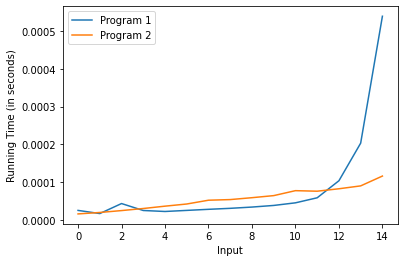
\includegraphics[width=0.75\textwidth]{./running_times.png}\\
    
    Interestingly, we see that program $2$ is faster than program $1$ for large values of $n$, the input size. The graph of runtime above suggests that this holds asymptotically. 
    
    \item Explain the discrepancies you see between Parts~\ref{itm:RAMtime} and \ref{itm:realtime}.  (Hint: What do we know about the relationship between the RAM and Word-RAM models, and why is it relevant to how efficiently the Python simulation runs?)  \\
    
    In part $2a$, we stated that both RAM-model running times were linear, and specifically that program $1$ was faster with a runtime of $4N+10$ compared to program $2$'s running time, $7N+14$. However, this is when we consider all mathematical operations as $O(1)$ time. The Python simulation in $2b$, however, shows that program $1$ in reality runs slower than program $2$, wit program $1$ looking almost exponential. This is because, in reality (practically), we cannot consider all mathematical operations as the same, or $O(1)$ time. Consider the fact that the approach to calculate running times in part $2a$ is $O(1)$ for line $8$ and $9$ in programs $1$ and $2$ respectively, regardless of if the number is large or small. In reality these calculations take significantly longer the larger the input number becomes. \\ 
    
    Importantly, consider the fact that program $1$ is a basic RAM model, meaning there are no bounds on the memory size. With the output beign $11^{2^N + 1}$, we have that as $N \to \infty$, it follows that $Output \to \infty$. Since the input is only restricted to the natural numbers, massive input values of $n$ are possible and can allow the operations computed in line $8$ of program $1$ to take (exponential) amounts of time. \\
    
    On the other hand, program $2$ can be thought of a WORD-RAM model, where the word length is $32$ such that all entries are less than $2^w = 2^{32}$. The purpose of the WORD-RAM model is specifically to reduce the possible input size and magnitude of the entries stored in memory, so that the mathematical operations are bounded. This can be observed perfectly in program $2$, where we see that the output is restricted $\mod 2^{32}$. This means that in line $9$, the size of the possible values for result at each of the $n$ iterations is restricted $\mod 2^{32}$ because of lines $10-12$ that implement the mod function, making the runtime much lower than program $1$ because (relatively) massive numbers are not being fed into the calculation in line $9$, making the runtime appear more linear in nature since the inputs are smaller and the assumption that these calculations are $O(1)$ isn't as far off. \\
    
    \item (optional\footnote{This problem won't make a difference between N, L, R-, and R grades.}) Give a theoretical explanation (using asymptotic estimates) of the shapes of the runtime curves you see in Part~\ref{itm:realtime}. You may need to do some research online and/or make guesses about how Python operations are implemented to come up with your estimates. \\
    
    In Python, multiplication operations on extremely large numbers are computed using Karatsuba's algorithm, which has a runtime of $O(x^{\log_2 3})$  for an $x$-bit integer. Consider program 1. We have that the for any input size $n$, the number inputted into the loop starting at line $7$ is $11^{2^n}$. Thus, the number of bits inputted is simply $\lfloor \log_2 11^{2^n} \rfloor + 1$. Then, using Karatsuba's algorithm, it follows that the runtime for program $1$ is $O\left ( \lfloor \log_2 11^{2^n} \rfloor + 1 \right)^{\log_2 3}$. We can simplify this to get a better idea of the runtime. We first remove the floor and proceed.
    
    $$
    O\left ( \lfloor \log_2 11^{2^n} \rfloor + 1 \right)^{\log_2 3}
    $$
    $$
     = O\left ( \log_2 11^{2^n} + 1 + 1 \right)^{\log_2 3}
    $$
    $$
     = O\left ( 2^n \times \log_2 11 + 2 \right)^{\log_2 3}
    $$
    $$
     = O\left ( 2^n \left(\log_2 11 + \frac{1}{2^{n-1}}\right) \right)^{\log_2 3}
    $$
    $$
     = O\left ( 2^{n \times \log_2 3} \times \left(\log_2 11 + \frac{1}{2^{n-1}}\right)^{\log_2 3} \right)
    $$
    $$
     = O\left ( 3^n \times \left(\log_2 11 + \frac{1}{2^{n-1}}\right)^{\log_2 3} \right)
    $$
    
    Now note that as $n \to \infty$ (asymptotically), $\left(\log_2 11 + \frac{1}{2^{n-1}}\right)^{\log_2 3} \to (\log_2 11)^{\log_2 3}$, which we can abstract away as a constant $c$. Thus, we have that the runtime for program $1$ is, after simplification, close to $O(3^n)$, which is exponential in nature and reflects the trend observed in the run time graph. \\
    
    However, for program $2$, note that because of the $\mod 2^{32}$ steps taken in lines $10-12$, it follows that the value of $result$ as input to the loop starting at line $8$ is always $\leq 2^{32}$. Thus, in the mathematical operations found in line $9$, the starting value is bounded. If Karatsuba's algorithm is used for integers at this size, then we have that the running time of any iteration (any therefore the entire program) is $O\left((\log_2 2^{32}\right)^{\log_2 3})$. This can be simplified.
    $$
    O\left((\log_2 2^{32}\right)^{\log_2 3})
    $$
    $$
    = O\left((32\right)^{\log_2 3}),
    $$ which is a constant time asymptotically. Even if Karatsuba's algorithm is not used in Python for numbers of this size, and the grade-school algorithm used instead, it still follows that the runtime is bounded at a particular constant value due to the only input to the loop being $\leq 2^{32}$. Thus, as $n \to \infty$, the runtime ascends linearly like in part $2a$ because we treat smaller mathematical operations as almost constant.
\end{enumerate}

\item (Simulating Word-RAM by RAM)  Show that for every Word-RAM program $P$, there is a RAM program $P'$ such that $P'$ halts on $x$ iff $P$ halts on $x$, and if they halt, then  $P'(x)=P(x)$ and 
       $$\Time_{P'}(x) = O\left(\Time_P(x)+n+w_0\right),$$
where $n$ is the length of $x$ and $w_0$ is the initial word size of $P$ on input $x$.  (This was stated without proof in Lecture Notes 7.) 

Your proof should use an {\em implementation-level} description, similar to our proof that RAM programs can be simulated by ones with at most $c$ registers.  Recall that Word-RAM programs have read-only variables $\memsize$ and $\wordlen$; you may want to start your simulation by calculating these variables as well as another variable representing $2^{\wordlen}$.  Then think about how each operation of a Word-RAM program $P$ can be simulated in a RAM program $P'$, taking care of any differences between their semantics in the Word-RAM model vs. the RAM model. Don't forget MALLOC! \\

SOLUTION: Suppose we have as stated a Word-RAM program $P$. We will then show that $\exists$ a RAM program $P'$ using only standard RAM-based operations that can simulate all unique operations of $P$. Furthermore, we can show that the runtime of the simulation $P'$ can be thought of in terms of the original program $P$. Specifically, 

$$\Time_{P'}(x) = O\left(\Time_P(x)+n+w_0\right),$$

where $n$ is the length of the input $x$ and $w_0$ is the initial word length. \\

Initialize the variables $zero = 0$ and $one = 1$. Note that first we must encode the input from the Word-RAM model into the RAM memory. First the input $x$ is given as a sequence of $n$ natural numbers, where each number $y \leq 2^{w_0} - 1$. We encode these input numbers of $x$ into memory locations $M[0], M[1], \dots, M[n-1]$, and initialize the variable $\inputlen = n$ such that we keep track of the size of the input. Then set the memory size, which in Word-RAM is $S$, but here will be $\memsize = \inputlen + zero$. Initializing these variables would take $O(n)$ time. Now, we must find the size of the word length value to be stored in $\w_0$ the first time for initialization. Note that as defined in the Word-RAM problem, 
$$w_0 = \lfloor \ \log \max\{\memsize, M[0], M[1], \dots, M[\memsize-1]\}\rfloor + 1$$

We must find this initial $w_0$. First, we must find the maximum value between the memory locations and the input. First, we can start by initializing a variable $max$ to be $\inputlen$. Then, we have a variable counter to keep track of when we reach the end of the list, which we initialize to $0$. We initialize a conditional GOTO loop, checking that $counter - n$ is not $0$, with the GOTO going to the line after the GOTO if the condition evaluates to True.  We start by indexing into the first element in memory, such as by using $M[counter]$. We can initialize a value called $offset$ to be $max - M[counter]$. We again have a nested conditional, that is, if $offset == 0$, we GOTO a line defined to reassign $max$. At this line, we assign $max = M[counter]$. If the conditional evaluates to false, however, we continue by simply incrementing counter. We compute $counter = counter + one$. Then, we finally have a line such as IF $ zero = 0$ GOTO the line of the outer loop that checked if $counter$ met conditions. This code would calculate the maximum of the input size and numbers stored in memory. Iterating through the stored $n$ values to find the maximum would be $O(n)$ time. 

Now that the max is stored in the $max$ variable, we use it to assign $w_0$. Assign a variable $two = 2$. We must find a RAM way of implementing the $\log$ function. We reintialize $counter = zero$. Then, we have a conditional GOTO to go to the line of the loop being initialized now. First, we reassign $max = max / two$. Then we increment counter again, by computing $counter = counter + one$. Then, we have a GOTO condition $IF zero = 0$ GOTO the outer conditional described above, which always evaluates to true. Thus, by the end of this loop, in the counter variable is the value of  

$$\lfloor \ \log \max\{\inputlen, M[0], M[1], \dots, M[\inputlen-1]\}\rfloor$$. We can then initialize $w_0 = counter + 1$. Now, we can calculate the actual maximum value that can be stored, which we wish to be some variable $max-word-size$ such that $max-word-size = 2^{w_0}$. We can do this by including two conditional GOTO's with a counter such that the first conditional is true if some variable equals $w_0$, much like described before, initializing a variable to $1$, and then multiplying and reassigning that variable by $two$ every time within the loop. This loop would take $w_0$ steps. 

Then, we would need to modify the operations themselves. Note that the only change would be that in the RAM model we would have to prevent numbers larger than $max-word-size - 1$, to have a bound similar to that in Word-RAM. This would be applicable for addition and multiplication. We need to redefine the operations themselves, that is, for every command $c$ in the Word-RAM problem that has addition or multiplication, we add a step after that checks if the number is bounded or not. Suppose the result of the operation is some value which we denote $output$. Specifically, we use a conditional GOTO, where the condition is $max-word-size - output = 0$. If this is true ($output > max-word-size$), then we GOTO a line which reassigns the $output$ by means of $output = max-word-size - 1$, to keep the bounds as required. This implementation should also be added for every command in $P$ to read or write memory, as we must first check that the index trying to be accessed is less than $\memsize$. \\

The last modification for the simulation would need to be the $MALLOC$ command in Word-RAM. Here, we simply reassign $\memsize = \memsize + 1$. The value at $M[\memsize - 1]$ should already be initialized to $zero$ because of the definition of a RAM program, but now we can access it! \\

Overall, the execution of this simulation of $P$ by $P'$ would be constant time for the modifications of the operations as well as $MALLOC$. Initially writing into memory and finding the $\max$ would be $O(N)$ time, finding $2^{w_0}$ would take $O(w_0)$ time, and we would still have to go through the $c$ commands for $P$ that would take $O\left(\Time_P(x)\right)$. Thus, the total runtime for execution would be as expected, 

$$\Time_{P'}(x) = O\left(\Time_P(x)+n+w_0\right),$$. 
\end{enumerate}


\end{document}
